\Section{Designing GCom middleware}

\paragraph{}{
	The GCom application is basically made up of three layers as
 we can see on figure \ref{fig:architecture}.
 Each layer has different responsibilities. The layers allow 
 making abstraction and shared out responsibilities.
}

\begin{figure}[!ht]
	\begin{center}
	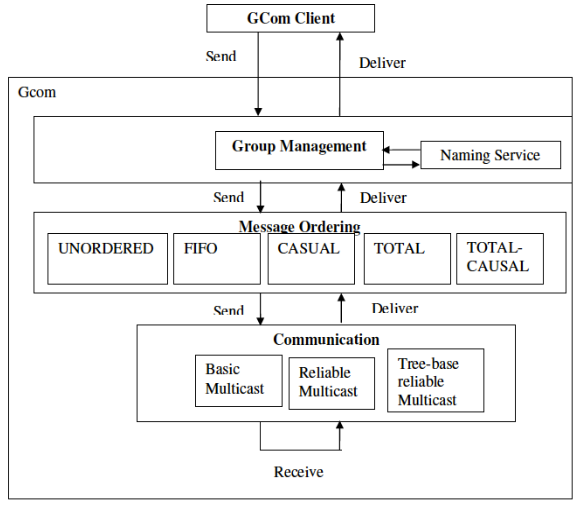
\includegraphics[width=0.7\textwidth]{figures/gcom_architecture.png}
	\end{center}
	\caption{Global architecture of GCom middleware}
	\label{fig:architecture}
\end{figure}

\paragraph{Group management}{
	The top layer is the part tasked with the group management.
 The group management elects a new leader, adds and removes
 members within the group, handles errors and notify processes
 about group changes. It is at this level a member of a group keeps
 track of other members. }

\paragraph{Message ordering}{
	The message ordering layer determines in which order
 messages are delivered to the next layer according to different
 strategies. For instance, we can order messages according to the
 "First In, First out" policy, use a causal order or a mix
 between two existing ordering like Total-Casual.
}

\paragraph{Communication}{
	The communication service is the lowest level. It deals
 with the Java RMI objects. It allows different type of
 communication like multicasting and, maybe, a tree based
 communication.  \newline
 Moreover, the debug interface will be mainly implemented here.
}

\paragraph{Debugging}{
	Additionally, the communication module offers an interface
 to set up how to simulate network latency and failures.
}

\paragraph{Naming service}{
	To get into the group, or at least ask to group to join,
 we need a service to solve how to find a group on the network.
 It is basically the entry point of the system.
 This is also the only centralized part of the system.
}

\Subsection{Comments}
	For the group management level it is important to consider
 how many members to keep track of in order to maintain
 scalability. Our first approach will be to hold all members
 but if time allows a solution where only a partial list is kept
 will be considered.

The implementation will be constructed such that every layer
as presented in above will be represented in the implementation
where no component knows of components on a layer above.
This way we keep modularity and simplicity.
Along with this, errors should propagate upwards until it can
be handled in a correct way. For example, a timeout in the 
communication layer should propagate to the group management layer
in order to e.g. inform others of a crashed member.

A final note for the structure of the product.
As Gcom is a middleware this will be built as an independent JAR
dependency so that when the chat application is constructed
Gcom acts as an external dependency imported as a JAR.
This will also make for a cleaner design and implementation
if these are properly separated.
